\section{Analysierungsphase}\label{sec:analyze}

\begin{figure}[htbp] 
	\centering
	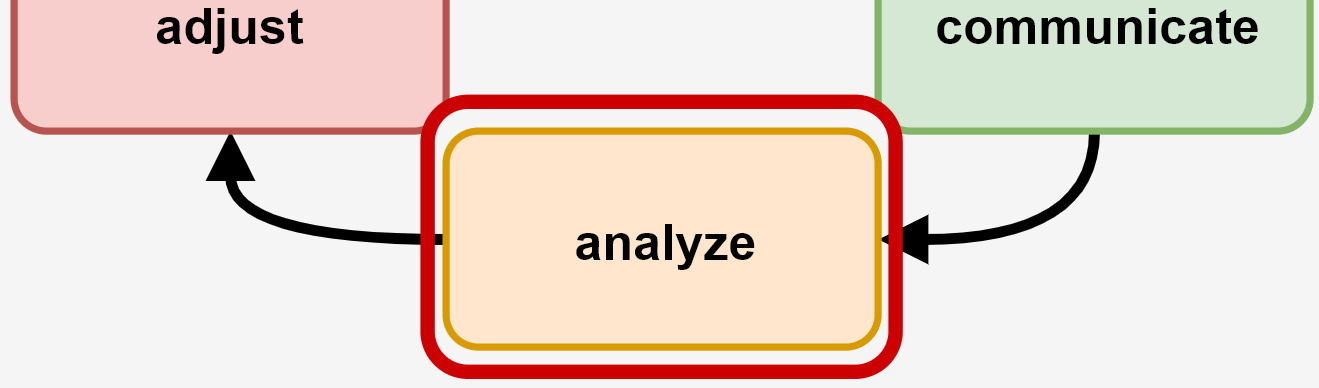
\includegraphics[width=0.75\textwidth]{contents/images/SmartGrazerSectionAnalyze}
	\caption{SmartGrazer: Auszug Analysierungsphase}
	\label{fig:SmartGrazerSectionAnalyze}
\end{figure}

Für die Analysephase ist es wichtig, Vergleichsdaten für die Antworten der Webseite zu haben. Aus diesem Grund wurde eine dritte Generator-Klasse implementiert, die fest definierte Anfragen erzeugt. Dieser Generator wird im Folgenden als ``Simpy'' bezeichnet. Die von Simpy generierten Payloads dienen der Initialisierung und Anpassung der Lebenspunkte der Element-Datenbank von SmartGrazer. Hierdurch ist es möglich, Smarty noch vor der ersten Generierungsrunde voreinzustellen.

Nachdem ein Payload an die SUT gesendet und die dazugehörige Antwort gepeichert wurde, beginnt die Analyse. Das Modul ``Annelysa'' übernimmt hierbei zwei Aufgaben. Zuerst wird anhand des Wissens aus der validen Anfrage und den Initialisierungs-Anfragen von Simpy die Position des Payloads bestimmt. Diese Position wird im weiteren Verlauf dazu verwendet, um nach dem zuletzt gesendeten Payload zu suchen. Die Position des Payloads ist wichtig, da Webseiten oft Benutzereingaben auf XSS-Angriffe durchsuchen und Elemente verändern oder entfernen, sodass nicht nach einer Übereinstimmung mit der Zeichenkette gesucht werden kann. Wenn die Position dem Analyse-Modul bekannt ist, kann anhand des originalen Payloads jedes Element einzeln untersucht und verglichen werden.

Annelysa ist zum jetzigen Stand der Implementierung darauf ausgelegt, dass die Webanwendung in jedem Fall den selben Seitenaufbau zurückliefert. Für Fälle, bei denen die Webseiten die bei Fehlern oder falschen Eingaben auf eine eigens dafür konzipierte Fehlerseite umgeleitet werden, ist SmartGrazer nicht ausgelegt.

\subsection{Textbasierte Suche} \label{ssec:textbase-search}

\begin{figure}[htbp] 
	\centering
	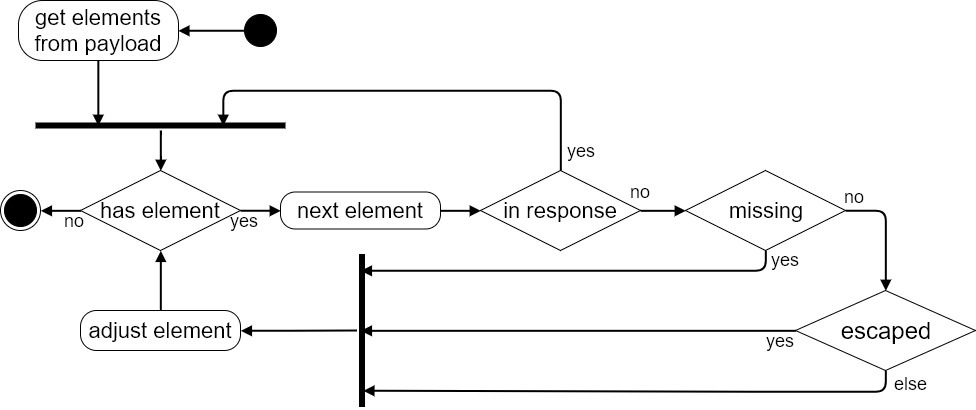
\includegraphics[width=0.9\textwidth]{contents/images/SmartGrazerTextBasedSearch}
	\caption{Ablaufdiagramm: Textbasierte Payload-Suche}
	\label{fig:textbasedsearch}
\end{figure}

Die bisherige Implementierung umfasst drei mögliche Szenarien der Webseiten-Antwort. Im ersten Fall wird die Payload-Zeichenkette ohne Modifikation vom Server reflektiert. Im zweiten Fall kann der Payload nicht direkt in der Antwort gefunden werden. Dies umfasst Elemente, welche durch die HTML-Entities-Kodierung ausgetauscht wurden. Besonders Zeichen, die Bestandteil von HTML oder JavaScript sind, werden durch diese Kodierung unbrauchbar. Der dritte Fall umfasst die Entfernung bestimmter Elemente aus dem Payload. Im zweiten und dritten Fall werden nach dem Erkennen eines veränderten oder fehlenden Elements, wie in Kapitel \ref{ssec:elementlifepoints} definiert, die Lebenspunkte verringert. Anschließend wiederholt sich die Suche für alle Elemente des im Generator gewählten Payloads.

Im optimalen Fall hat das \ac{SUT} keine Änderungen vorgenommen und den Payload reflektiert, sodass für kein Element die Lebenspunkte angepasst werden müssen. Sobald ein Element in der Antwort jedoch verändert oder entfernt wurde, gilt der Test als fehlgeschlagen. Nichtsdestotrotz werden alle Elemente der Antwort gesucht, da jede erkannte Änderung zu einer verbesserten Generierung in der nächsten Runde beiträgt.

\subsection{Ausführung des Payloads}\label{AusführungDesPayload}

Als weitere Testinstanz wird versucht, erfolgreich eingeschleuste Payloads auszuführen. Ein Payload, der zwar reflektiert worden ist, jedoch keine Auswirkung auf die Webseite hat, wird als Falsch-Positiv-Meldung bezeichnet.

% Warum Ausführung sinnvoll
Solche Payloads werden vom Programm als valide bzw. erfolgreich bewertet, bringen dem Nutzer bzw. Tester aber keinen Mehrwert. Wenn der gelieferte Payload bereits ausgeführt und getestet worden ist, kann der Tester eine erweiterte Version des Payloads mit alternativem JavaScript-Code erstellen, der mit Sicherheit funktioniert.

% Wie wird es gemacht
Realisiert wird das Testen der Ausführung durch Selenium\footnote{\url{http://www.seleniumhq.org/}}. Dieses Framework ist für automatisierte Browsertests konzipiert. Das Testen eines Payloads wird durch das vorherige Speichern der Antwortseite ermöglicht. Durch das automatische Laden der Antwortseite im Webbrowser wird zunächst das \ac{DOM} erstellt und anschließend der JavaScrip-Interpreter ausgelöst. Falls sich der Payload in einem aktiven JavaScript-Kontext befindet, wird dieser ausgeführt. Wurde nach dem Laden der Seite ein JavaScript Pop-up geöffnet, gilt der Payload als ausgeführt und ist somit funktionsfähig.

% Warum ggf. besser die Response zu rendern und nicht die gespeicherten Daten
Eine Ausführung zur Laufzeit, d.h. bei der ersten Anfrage an die Webanwendung, wäre der bisherigen Methode vorzuziehen. Jedoch ist dies bisher nicht möglich, da die technische Entwicklung noch nicht ausgereift ist.
Die Ausführung zur Laufzeit hat im Wesentlichen zwei Gründe:

\begin{enumerate}
	\item Bei stark dynamischen Webseiten wird JavaScript-Code aus Dateien eingebunden. Diese JavaScript-Quelltexte werden beim Speichern der Antwortseite nicht kopiert und fehlen dementsprechend beim späteren Laden der Webseite im Browser.
	\item Eine Auswertung zur Laufzeit könnte unnötige Anfragen an die Webseite reduzieren. Im Falle einer ``Wortverdoppelung'' (Bsp.: javajavascriptscript) wird durch Entfernen des Wortes ``javascript'' der Payload aktiviert und dadurch eventuell ausgeführt. Die bisherige Implementierung von SmartGrazer erkennt eine Veränderung und überspringt somit die Ausführung des betroffenen Payloads.
	Dieser Fall würde zu weiteren Anfragen führen, obwohl bereits ein Payload funktionsfähig war.
\end{enumerate}